% ================================================
% 文件: 01_接收机基础.tex
% 章节: 第6章 接收机基础
% 所属部分: 接收机技术
% 版本: v1.0
% ================================================
% 本章目录结构（树状）:
% \chapter{接收机基础}
% ├── \section{接收机基本原理}
% ├── \section{接收机主要技术指标}
% ├── \section{接收机类型与分类}
% ├── \section{直接放大式接收机}
% ├── \section{外差原理}
% └── \section{超外差式接收机原理}
% ================================================

\chapter{接收机基础}
\label{chap:receiver_fundamentals}

\section{接收机基本原理}
\label{sec:receiver_principle}

接收机是一种将无线电信号转换为可感知信号（如音频、视频）的电子设备。其基本工作流程为：

\begin{itemize}
    \item \textbf{接收}：通过天线捕获空间中的无线电波
    \item \textbf{选择}：通过调谐电路选择特定频率的信号
    \item \textbf{放大}：通过放大器增强信号强度
    \item \textbf{解调}：从载波中提取原始调制信号
    \item \textbf{输出}：将解调后的信号转换为音频或视频输出
\end{itemize}

接收机的核心任务是在噪声环境中可靠地恢复原始信号。

\section{接收机主要技术指标}
\label{sec:receiver_specifications}

评价接收机性能的主要指标包括：

\begin{itemize}
    \item \textbf{灵敏度}：接收机能够检测到的最小信号强度，通常用dBm表示
    \item \textbf{选择性}：接收机区分相邻信道信号的能力，用带宽或Q值表示
    \item \textbf{增益}：接收机对信号的放大能力，用dB表示
    \item \textbf{噪声系数}：接收机自身产生的噪声大小，用dB表示
    \item \textbf{失真}：信号经过接收机后产生的畸变程度
    \item \textbf{动态范围}：接收机能够处理的信号强度范围
    \item \textbf{镜像抑制}：超外差接收机抑制镜像频率干扰的能力，用dB表示，通常要求大于60dB
\end{itemize}

\section{接收机类型与分类}
\label{sec:receiver_classification}

接收机可按多种方式分类：

\begin{itemize}
    \item \textbf{按工作原理}：直接放大式、超外差式、直接转换式
    \item \textbf{按调制方式}：AM接收机、FM接收机、SSB接收机
    \item \textbf{按工作频段}：长波、中波、短波、超短波、微波接收机
    \item \textbf{按用途}：广播接收机、通信接收机、雷达接收机、导航接收机
\end{itemize}

\section{直接放大式接收机}
\label{sec:direct_amplification_receiver}

直接放大式接收机直接对射频信号进行放大，然后解调。

直接放大式收音机的工作原理如下：从天线上传下来的各射频信号到达调谐电路，由调谐电路的谐振作用，选择了其中某一个射频信号，经射频放大器放大后，再经调谐电路的调谐，于是输入到检波器，由检波器将射频电压变换为音频电压，再经音频放大器放大，输入到扬声器。

\begin{figure}[htbp]
    \centering
    \begin{tikzpicture}[
        block/.style={rectangle, draw, fill=blue!20, 
            text width=4.5em, text centered, minimum height=2.5em},
        line/.style={draw, -latex'},
        signal/.style={coordinate},
        node distance=0.6cm
    ]
    
    % 节点定义
    \node[signal] (input) {};
    \node[block, right=of input] (tuner1) {调谐电路};
    \node[block, right=of tuner1] (rfamp) {射频放大器};
    \node[block, right=of rfamp] (tuner2) {调谐电路};
    \node[block, right=of tuner2] (detector) {检波器};
    \node[block, right=of detector] (afamp) {音频放大器};
    \node[signal, right=of afamp] (output) {};
    
    % 连线
    \draw[line] (input) -- (tuner1);
    \node[above=0.3cm of input] (rf_label) {\small 射频信号};
    \draw[line] (tuner1) -- (rfamp);
    \draw[line] (rfamp) -- (tuner2);
    \draw[line] (tuner2) -- (detector);
    \draw[line] (detector) -- (afamp);
    \draw[line] (afamp) -- (output);
    \node[above=0.3cm of output] (af_label) {\small 音频信号};
    
    % 功能说明标签
    \node[below=0.4cm of tuner1, font=\small] {选择信号};
    \node[below=0.4cm of rfamp, font=\small] {放大信号};
    \node[below=0.4cm of tuner2, font=\small] {选择信号};
    \node[below=0.4cm of detector, font=\small] {解调音频};
    \node[below=0.4cm of afamp, font=\small] {驱动扬声器};
    
    \end{tikzpicture}
    \caption{直接放大式接收机结构框图}
    \label{fig:direct_amplification_block}
\end{figure}

从框图中可以看出：自天线电路到检波级，对于原来电信的频率和波形一直没有改变；而且每多加一级射频放大，可以多增加一个调谐电路。

我们知道：调谐电路越多，或者调谐电路的调谐特性越尖锐，收音机的选择性必越高。因此，要装置一架高度选择性的直线放大式收音机，就必需增加调谐电路。但是，调谐电路越多，将使收音机的构造格外复杂，调节越加困难。

优点：
\begin{itemize}
    \item 结构简单
    \item 成本低
\end{itemize}

缺点：
\begin{itemize}
    \item 选择性差
    \item 灵敏度低
    \item 稳定性差
\end{itemize}

直接放大式接收机主要用于简单的矿石收音机和早期的广播接收机。

\section{调谐电路特性}
\label{sec:tuning_circuit_characteristics}

调谐电路是接收机的核心组成部分，其特性直接影响接收机的性能。

\subsection{频率特性曲线}

图\ref{fig:tuning_characteristics}展示了两种不同特性的调谐电路：

\begin{figure}[htbp]
    \centering
    \begin{tikzpicture}[
        axis/.style={->, >=stealth', line width=0.8pt},
        curve/.style={line width=1.2pt},
        node distance=1cm
    ]
    
    % 坐标轴
    \draw[axis] (0,0) -- (8,0) node[right] {频率};
    \draw[axis] (0,0) -- (0,5) node[above] {增益};
    
    % 高选择性曲线 (尖锐)
    \draw[curve, red] plot[smooth] coordinates {
        (1,0.2) (2,0.5) (3,1.5) (4,4.5) (5,1.5) (6,0.5) (7,0.2)
    } node[above right, red, font=\small] {高选择性};
    
    % 低选择性曲线 (平缓)
    \draw[curve, blue, dashed] plot[smooth] coordinates {
        (0.5,0.8) (1.5,1.5) (2.5,2.5) (4,3.8) (5.5,2.5) (6.5,1.5) (7.5,0.8)
    } node[above right, blue, font=\small, dashed] {低选择性};
    
    % 标记谐振频率
    \draw[dashed, gray] (4,0) -- (4,4.5) node[below, gray, font=\small] {$f_c$};
    \node[below] at (4,0) {谐振频率};
    
    % 标记通频带
    \draw[dashed, gray] (2.5,1) -- (5.5,1);
    \node[below] at (4,1) {$\Delta f$ 通频带};
    
    \end{tikzpicture}
    \caption{两种调谐电路的频率特性曲线：(a) 高选择性（尖锐曲线）；(b) 低选择性（平缓曲线）}
    \label{fig:tuning_characteristics}
\end{figure}

\begin{itemize}
    \item \textbf{高选择性电路（图a）}：曲线非常尖锐，通频带（包括谐振频率左右的一段频带）很窄。优点是选择性很好，能有效区分相邻频率的信号；缺点是通频带过窄会引起频率畸变。
    
    \item \textbf{低选择性电路（图b）}：曲线比较平缓，通频带较宽。优点是频率畸变小，信号保真度高；缺点是选择性较差，容易受到相邻频道的干扰。
\end{itemize}

\subsection{选择性与频率畸变的权衡}

要使直接放大式收音机的选择性优良，调谐电路的通频带必须尽可能窄。然而，通频带越窄，将引起频率畸变越大。这是一个基本的权衡关系。

频率畸变会导致信号的某些频率分量被衰减，造成声音失真。对于音频信号来说，这会使声音变得不自然。

\subsection{直接放大式电路的局限性}

由于直接放大式电路的特性关系，存在以下问题：

\begin{itemize}
    \item \textbf{放大率不均匀}：对于各频段的放大率极不均匀
    \item \textbf{短波接收性能差}：接收短波波段的电信时，收音机电路的选择性随着频率的提高而迅速降低
    \item \textbf{灵敏度下降}：放大级的放大率减退，使收音机的选择性及灵敏度格外低落
\end{itemize}

这些局限性导致直接放大式接收机逐渐被性能更优越的超外差式接收机所取代。

\section{外差原理}
\label{sec:heterodyne_principle}

外差原理（Heterodyne Principle）是无线电通信中的基本原理，由加拿大工程师Reginald Fessenden于1901年提出。该原理是超外差接收机架构的理论基础。

\subsection{外差原理的原理与示例}

外差原理的核心思想是：将两个不同频率的信号在非线性器件（如二极管、晶体管、电子管）中混合，会产生新的频率分量。

\subsubsection{数学基础}

假设两个输入信号的瞬时值分别为：
\[ v_1(t) = A_1 \cos(2\pi f_1 t) \]
\[ v_2(t) = A_2 \cos(2\pi f_2 t) \]

在非线性器件中混合后，输出信号将包含以下频率分量：
- 原频率分量：\( f_1 \) 和 \( f_2 \)
- 和频分量：\( f_1 + f_2 \)
- 差频分量：\( |f_1 - f_2| \)

其中，差频分量是外差原理中最常用的分量。

\subsubsection{通俗解释}

当两个频率不同的电压输入到同一电路时，将得到第三个频率的电压。如果这第三个频率的电压经电子管检波器检波，在检波器阳极电路中将出现两个电压的频率的差数电压，即差频电压。

譬如第一个电压 \( f_1 \) 的频率是24赫兹，第二个电压 \( f_2 \) 的频率是22赫兹，在检波器阳极电路中的差频电压，将为 \( 24 - 22 = 2 \) 赫兹。

\subsection{外差原理的应用}

外差原理的主要应用包括：

\begin{itemize}
    \item \textbf{频率变换}：将高频信号转换为较低的中频信号，便于放大和处理
    \item \textbf{解调}：通过与本地振荡信号混合，提取调制信号
    \item \textbf{频率合成}：生成新的频率信号
    \item \textbf{差拍检波}：用于接收CW（连续波）信号，如莫尔斯电码
\end{itemize}

\subsubsection{差拍检波与CW接收}

差拍检波（Beat Detection）是外差原理在连续波（CW）通信中的经典应用。CW信号是一种单一频率的等幅波，本身不携带音频信息，需要通过差拍原理将其转换为可听信号。

工作原理：
1. **接收信号**：电台发射的CW信号（如莫尔斯电码的点和划）
2. **本地振荡器**：接收机内部产生一个频率非常接近接收信号的本地振荡信号
3. **差拍产生**：两个信号在非线性器件中混合，产生差频信号
4. **音频输出**：当差频落在音频范围内（如几百赫兹到几千赫兹），就能听到"滴答"声

例如：
- 接收CW信号频率：\( f_{signal} = 7050 \) kHz
- 本地振荡频率：\( f_{local} = 7050.8 \) kHz
- 差拍频率：\( |7050.8 - 7050| = 0.8 \) kHz = 800 Hz

这个800Hz的差拍信号就是我们听到的CW音频信号。

\begin{figure}[htbp]
    \centering
    \begin{tikzpicture}[
        block/.style={rectangle, draw, fill=blue!20, 
            text width=5em, text centered, minimum height=2em},
        line/.style={draw, -latex'},
        signal/.style={coordinate},
        node distance=0.5cm
    ]
    
    \node[signal] (input) {};
    \node[block, right=of input] (mixer) {混频器};
    \node[block, above=of mixer] (localosc) {本地振荡器};
    \node[block, right=of mixer] (filter) {音频滤波器};
    \node[block, right=of filter] (amp) {音频放大器};
    \node[signal, right=of amp] (output) {};
    
    \draw[line] (input) -- (mixer) node[above, midway, font=\small] {CW信号};
    \draw[line] (localosc) -- (mixer) node[right, midway, font=\small] {本振信号};
    \draw[line] (mixer) -- (filter) node[above, midway, font=\small] {差拍信号};
    \draw[line] (filter) -- (amp);
    \draw[line] (amp) -- (output) node[above, midway, font=\small] {音频输出};
    
    \end{tikzpicture}
    \caption{差拍检波原理框图}
    \label{fig:beat_detection}
\end{figure}

差拍检波的优点：
\begin{itemize}
    \item \textbf{灵敏度高}：能检测非常微弱的CW信号
    \item \textbf{选择性好}：通过调整本振频率精确选择信号
    \item \textbf{简单实用}：电路结构相对简单
\end{itemize}

\subsection{差频产生的物理过程}

由于两个不同频率的电压，在某一些时间，因为它们的方向相同而相加（在b点相加最大）；在另一些时间，因为它们的方向相反而相减（在a点和c点相减最大）。因此，合成的电压的波幅就不再相等。波幅在每秒钟内升降的周数，将等于它们的频率的差数。

\begin{figure}[htbp]
    \centering
    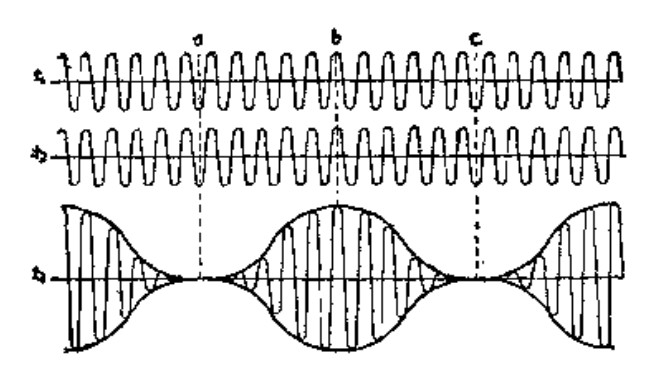
\includegraphics[width=0.8\textwidth]{Images/beat_frequency_wave.jpg}
    \caption{两个不同频率信号合成后的差频作用}
    \label{fig:beat_frequency_wave}
\end{figure}

由于电子管检波器的阳极平均电流是按第三个频率的电压的波幅而变动的，所以阳极电路出现了差频电压。

\subsubsection{超外差式收音机中的差频应用}

在超外差式收音机中，第一个电压就是输入到变频器的外来广播电台的已调制射频电信电压，第二个电压是由收音机里的高频振荡电路所产生的高频电压。这个高频振荡器所以叫做本机振荡器。

如果外来射频电压的频率为1000千赫，本机振荡器所产生的高频电压的频率为1465千赫，它们同时输入到变频器，由变频器转换后所输出的电压，它的频率将为两个电压的频率的差数，即 \( 1465 - 1000 = 465 \) 千赫。这个差频，就是我们所谓中频。

\begin{figure}[htbp]
    \centering
    \begin{tikzpicture}[
        block/.style={rectangle, draw, fill=blue!20, 
            text width=5em, text centered, minimum height=2em},
        line/.style={draw, -latex'},
        signal/.style={coordinate},
        node distance=0.5cm
    ]
    
    \node[signal] (input) {};
    \node[block, right=of input] (mixer) {变频器};
    \node[block, below=of mixer] (localosc) {本机振荡器};
    \node[block, right=of mixer] (output) {中频输出};
    
    \draw[line] (input) -- (mixer) node[above, midway, font=\small] {射频信号 (1000kHz)};
    \draw[line] (localosc) -- (mixer) node[left, midway, font=\small] {本振信号 (1465kHz)};
    \draw[line] (mixer) -- (output) node[above, midway, font=\small] {中频信号 (465kHz)};
    
    \end{tikzpicture}
    \caption{变频器工作情形}
    \label{fig:mixer_operation}
\end{figure}

\subsection{外差与超外差的区别}

\begin{enumerate}
    \item \textbf{外差接收机}：早期实现，中频不固定，随接收频率变化
    \item \textbf{超外差接收机}：现代主流架构，使用固定中频，性能更稳定
\end{enumerate}

"超外差"（Superheterodyne）中的"超"（Super）表示这种架构超越了早期的简单外差技术，通过固定中频实现了更高的灵敏度和选择性。

\section{超外差式接收机原理}
\label{sec:superheterodyne_principle}

超外差式接收机是目前应用最广泛的接收机架构，其核心原理是将不同频率的射频信号转换为固定的中频信号进行处理。

工作流程：
1. \textbf{调谐}：选择所需的射频信号
2. \textbf{变频}：将射频信号与本地振荡器信号混合，产生中频信号
3. \textbf{中频放大}：对中频信号进行高增益放大
4. \textbf{解调}：从中频信号中提取音频信号
5. \textbf{音频放大}：放大音频信号驱动扬声器

中频频率通常选择为455kHz（AM广播）或10.7MHz（FM广播）。

超外差式收音机先将接收到的射频信号电压，由一个所谓变频器变换成为一定的高频，即中频（因为它的频率比原来信号的频率低，比音频高，所以叫做中间频率，简称中频），经中频放大器放大后，再输入到检波器；而且中频放大级是超外差式收音机的主要增益部分。

相比直接放大式接收机，超外差式具有以下优点：

\begin{itemize}
    \item \textbf{灵敏度高}：中频放大器可工作在最佳频率，获得高增益
    \item \textbf{选择性好}：固定中频便于使用高性能滤波器
    \item \textbf{稳定性好}：本振频率相对稳定，避免漂移影响
    \item \textbf{通用性强}：同一中频放大器可接收不同频率信号
\end{itemize}

\subsection{超外差式接收机的核心优势}

超外差式收音机接收任何一个频率的电信，都使它变换成为同一中频，所以超外差式收音机没有直接放大式收音机那些缺点。

\subsubsection{优势一：音质优良}

由于频率已经固定，它的调谐电路的调谐特性就无需十分尖锐。那就是说，它可能获得充分宽广的畅通频带，从而减少频率畸变，所以超外差式收音机的音质比较好。

\subsubsection{优势二：放大效率高}

因为频率降低，中频放大级的放大效率得到了充分的发挥。一级中频放大器的增益要比一级射频放大器高出若干倍，尤其接收短波波段电信，格外显出了它的优越性。

\subsubsection{优势三：放大率均匀}

由于中频放大器只放大一定的中频电压，因此对于各频带的电信都能获得一律的放大率。

\subsubsection{结构优势}

由于这种种原因，所以超外差式收音机能够发挥那些直接放大式收音机所没有的特长；而且即使在超外差式收音机里装置好几级中频放大器，也不会有很大的困难。

\begin{figure}[htbp]
    \centering
    \begin{tikzpicture}[
        block/.style={rectangle, draw, fill=blue!20, 
            text width=4.5em, text centered, minimum height=2.5em},
        line/.style={draw, -latex'},
        signal/.style={coordinate},
        node distance=0.6cm
    ]
    
    % 节点定义
    \node[signal] (input) {};
    \node[block, right=of input] (tuner) {调谐电路};
    \node[block, right=of tuner] (mixer) {变频器};
    \node[block, above=of mixer, node distance=0.8cm] (localosc) {本地振荡器};
    \node[block, right=of mixer] (ifamp) {中频放大器};
    \node[block, right=of ifamp] (detector) {检波器};
    \node[block, right=of detector] (afamp) {音频放大器};
    \node[signal, right=of afamp] (output) {};
    
    % 连线
    \draw[line] (input) -- (tuner);
    \node[above=0.3cm of input] (rf_label) {\small 射频信号};
    \draw[line] (tuner) -- (mixer);
    \draw[line] (localosc) -- (mixer);
    \node[right=0.2cm of localosc] (lo_label) {\small 本振信号};
    \draw[line] (mixer) -- (ifamp);
    \node[above=0.3cm of mixer] (if_label) {\small 中频信号};
    \draw[line] (ifamp) -- (detector);
    \draw[line] (detector) -- (afamp);
    \draw[line] (afamp) -- (output);
    \node[above=0.3cm of output] (af_label) {\small 音频信号};
    
    % 功能说明标签
    \node[below=0.4cm of tuner, font=\small] {选择信号};
    \node[below=0.4cm of mixer, font=\small] {变频为中频};
    \node[above=0.4cm of localosc, font=\small] {产生本振};
    \node[below=0.4cm of ifamp, font=\small] {高增益放大};
    \node[below=0.4cm of detector, font=\small] {解调音频};
    \node[below=0.4cm of afamp, font=\small] {驱动扬声器};
    
    \end{tikzpicture}
    \caption{超外差式接收机结构框图}
    \label{fig:superheterodyne_block}
\end{figure}